% ICML 2024 two-column proposal.
% Compile: tectonic proposal.tex
\documentclass{article}

\usepackage{microtype}
\usepackage{graphicx}
\usepackage{subfigure}
\usepackage{booktabs}
\usepackage{hyperref}
\usepackage{url}
\usepackage{amsmath,amssymb,amsfonts}
\usepackage{algorithm}
\usepackage{algorithmic}
\usepackage{multirow}
\usepackage{tikz}
\usetikzlibrary{positioning,arrows.meta,shapes,fit,calc}
\usepackage[accepted]{icml2024}

\icmltitlerunning{Camera-Aware FL for Robotic Manipulation}

\begin{document}

\twocolumn[
\icmltitle{Camera-Aware Federated Manipulation:\\
Decoupling Task-Level Geometry from Federated-Level Camera Heterogeneity}

\begin{icmlauthorlist}
\icmlauthor{Siwon Kim}{dgist}
\icmlauthor{Haeun Yun}{dgist}
\icmlauthor{Jinhyung Lee}{dgist}
\icmlauthor{Gihyun Baek}{dgist}
\end{icmlauthorlist}

\icmlaffiliation{dgist}{DGIST}
\icmlkeywords{federated learning, robotic manipulation, diffusion policy,
camera heterogeneity, representation alignment, foundation models}
\vskip 0.3in
]

% Authors share contact via DGIST; email is intentionally omitted here.
% Define the corresponding-author text directly so the icml2024 style
% does not emit empty <> brackets or the AUTHORERR placeholder.
\makeatletter
\gdef\icmlcorrespondingauthor@text{Siwon Kim, Haeun Yun, Jinhyung Lee, Gihyun Baek}
\makeatother

\printAffiliationsAndNotice{}

\begin{abstract}
The FLAME federated-manipulation benchmark fails on \emph{Insert Peg}
and \emph{Scoop} (0\% across every aggregator) for two
\emph{orthogonal} reasons that the existing literature blends
together. \textbf{Task-level}, contact-rich manipulation needs
metric 3-D understanding that no monocular front-view encoder can
recover from $\sim$100 demos. \textbf{Federated-level}, each
client observes the same task through a different camera
projection $(K_c, T_c)$, so a 2-D image encoder is forced to
absorb both manipulation semantics and camera-dependent geometry
through a single shared parameter set --- which makes any
aggregation, FedAvg or otherwise, unstable. We propose a recipe
that addresses each axis with a different mechanism.
\emph{(i)} A frozen DINOv3 + Depth-Anything backbone with
client-side LoRA, lifted into a small client-local voxel volume
using each client's known $K_c$ and $T_c$ (a VolumeDP-lite
encoder), addresses the task axis by exposing metric depth.
\emph{(ii)} The same volumetric lift, applied \emph{before} any
parameter is communicated, addresses the federated axis by
realigning client observations into a shared world-frame
representation; the server therefore aggregates lightweight
modules over a geometrically normalised feature space rather than
over heterogeneous 2-D projection distributions.
\emph{(iii)} A 16-mode replay-ceiling sweep is included as a
\emph{controllability diagnostic} (not a federated component) to
fix JP-servo $g\!=\!20$ as the action interface across all
methods, so that subsequent comparisons isolate representation and
aggregation effects. We then specify four aggregation variants
(global, shared encoder / local decoder, local adapter / shared
decoder, FedRep-style staged) and a corresponding evaluation
protocol that reports not only mean SR but worst-client SR and
client variance, the metrics that actually matter for federated
deployment.
\end{abstract}

\section{Introduction}
\label{sec:intro}

FLAME~\cite{flame2025} unifies four RLBench manipulation tasks under
a federated protocol with $4 \!\times\! 420 \!\times\! 100$ demonstrations.
Tab.~\ref{tab:flame} shows the canonical CNN+MLP+FedAvg recipe
collapses on \emph{Insert Peg} and \emph{Scoop} regardless of which
aggregator (FedAvg, FedAvgM, FedOpt, Krum) is used. Most prior work
on this benchmark has tried to fix this by changing the
\emph{aggregator}. We argue this is the wrong axis: the benchmark
collapses because \emph{the model never received a fair geometry
budget}, not because the aggregator was poorly chosen.

\paragraph{Two orthogonal sources of difficulty.}
We decompose FLAME into two axes that the literature usually mixes:

\noindent\textbf{Task-level (geometric).} \emph{Insert} and
\emph{Scoop} require sub-mm 3-D understanding to bridge contact
phases. Even strong centralised manipulation models that operate on
2-D front views (RVT-2 \cite{rvt2}, SAM2Act \cite{sam2act}) rely on
multi-view geometry or auxiliary 3-D supervision precisely because a
single monocular front view does not provide metric depth.

\noindent\textbf{Federated-level (camera heterogeneity).}
Each client observes its workspace through a front camera with its
\emph{own} intrinsics $K_c$ and mounting pose $T_c$, perturbed
across institutions. A 2-D image encoder shared by FedAvg has to
average over models that have learned, on each client, a different
mapping from world geometry to image pixels. The aggregator is
asked to be robust to a confound that a smarter representation
could simply remove.

\paragraph{Our approach: two ideas, deliberately separated.}
We propose two architectural ideas that address the two axes
independently. Their effects are additive, but their FL benefits
come from different mechanisms, and we keep them decoupled
throughout the proposal so that each can be ablated, accepted, or
rejected on its own evidence.

\noindent\textbf{Idea A --- Foundation backbone with depth prior +
LoRA-only aggregation (\S\ref{sec:idea-a}).} A frozen DINOv3
\cite{dinov2} + Depth-Anything \cite{depthanything} backbone gives
the policy two things monocular RGB does not provide on its own:
self-supervised semantic features and a metric depth prior. The
backbone is byte-identical across clients and \emph{never
aggregated}; only LoRA \cite{lora} adapters of rank
$r\!\in\!\{4,8\}$ in the last attention blocks are trainable. The
\emph{FL contribution} of Idea A is not ``depth helps the task''
(though it does); it is that the encoder's drift surface is
collapsed to a small set of LoRA adapters, removing the dominant
client-drift source that every FL aggregator must otherwise absorb.

\noindent\textbf{Idea B --- Camera-aware world-frame lifting using
client-private $(K_c, T_c)$ (\S\ref{sec:idea-b}).} Each client uses
its own intrinsics $K_c$ and base extrinsic $T_c$ --- which it
already knows from the camera SDK and a one-time workspace
calibration --- to project image features into a world-aligned
voxel volume \emph{before} any parameter is communicated. The
\emph{FL contribution} of Idea B is representation alignment: the
aggregation surface is moved from heterogeneous 2-D camera-frame
features (where FedAvg interpolates between incompatible
projections) to aligned 3-D world-frame features (where averaging
is well-posed). $(K_c, T_c)$, the depth map, and the voxel volume
are local-only; nothing geometric crosses the network
(Fig.~\ref{fig:arch}).

\noindent The two ideas are complementary but \emph{independent}:
Idea A can be deployed without Idea B (a LoRA-only foundation
encoder, no voxel lift), Idea B without Idea A (camera-aware
lifting on top of a from-scratch encoder), or both together. Our
P2 ablation (\S\ref{sec:plan}) is designed to attribute the gain
to each separately.

\paragraph{Action interface as diagnostic, not contribution.}
We also run a 16-mode replay-ceiling sweep on the demonstration data
(Tab.~\ref{tab:ceiling}) and adopt JP-servo $g\!=\!20$ as the
universal action interface across all methods. We deliberately
position this analysis as a \emph{controllability diagnostic}, not
as a federated-learning contribution: an unreplayable action
interface would confound representation and aggregation
comparisons; fixing it lets us isolate the effects we actually want
to study (\S\ref{sec:diagnostic}).

\paragraph{Contributions.}
\textbf{(C1)} A decomposition of FLAME difficulty into
\emph{task-level} 3-D geometry deficiency and \emph{federated-level}
camera-induced client heterogeneity, with separate experimental
axes for each.
\textbf{(C2 --- Idea A)} A foundation-vision FL front end (frozen
DINOv3 + Depth-Anything + LoRA-only adapters) whose \emph{FL
contribution} is not ``depth helps manipulation'' but ``the
encoder's drift surface is collapsed to a small set of adapters'',
giving a $\sim\!10\!\times$ communication reduction and removing
the dominant source of client drift that aggregators must
otherwise absorb.
\textbf{(C3 --- Idea B)} A camera-aware world-frame voxelisation
that uses client-private $(K_c, T_c)$ to align heterogeneous
camera observations \emph{before} aggregation. The FL contribution
is representation alignment: the server averages over geometrically
normalised features rather than over incompatible 2-D projection
distributions. Camera parameters, depth, and voxels are
local-only; this is communication-free side information.
\textbf{(C4)} An aggregation-scope study tailored to the two
ideas: global-everything, shared encoder / local decoder, local
geometry adapter / shared decoder, and FedRep-style staged
personalisation \cite{fedrep}. We hypothesise that Ideas A and B
\emph{together} shrink the gap between FedAvg, FedProx, and
SCAFFOLD by removing the heterogeneity those algorithms exist to
absorb --- so the contribution becomes ``an aggregation surface
that no longer needs a heavy aggregator''.
\textbf{(C5)} A replay-ceiling controllability diagnostic that
fixes a fair action interface (JP-servo $g\!=\!20$) before any
representation or FL comparison, identified as the only mode
exceeding 0.8 SR on every task at oracle level.

\begin{table}[h]
\centering
\small
\caption{FLAME baselines~\cite{flame2025}. \emph{Insert} and
\emph{Scoop} collapse to 0\% under every aggregator, even before
camera shift is added.}
\label{tab:flame}
\begin{tabular}{lcccc}
\toprule
Method & Slide & Close & Peg & Scoop\\
\midrule
FedAvg  & 0.24 & 0.84 & 0.00 & 0.00\\
FedAvgM & 0.00 & 0.54 & 0.00 & 0.00\\
FedOpt  & 0.28 & 0.70 & 0.00 & 0.00\\
Krum    & 0.10 & 0.86 & 0.00 & 0.00\\
\bottomrule
\end{tabular}
\end{table}

\section{Problem Analysis}
\label{sec:problem}

\subsection{Task-Level: Geometry Deficiency}
\label{sec:problem-task}
Manipulation tasks involving contact require the policy to estimate
metric distance between gripper and object: how far to descend, how
far to advance, when to close the gripper. From a single front
RGB view, this estimation is ill-posed because object size and
distance are coupled. Depth-prior research (Depth-Anything
\cite{depthanything}) and 3-D-aware manipulation policies (RVT-2
\cite{rvt2}, SAM2Act \cite{sam2act}, VolumeDP \cite{volumedp2026})
all converge on the same conclusion: explicit 3-D structure is
necessary, not optional, for sub-mm precision tasks. The 0\% SR of
the FLAME baseline on \emph{Insert} and \emph{Scoop} is a direct
expression of this constraint, independent of whether the training
is centralised or federated.

\subsection{Federated-Level: Camera-Induced Heterogeneity}
\label{sec:problem-fl}
Different clients see the workspace through different cameras.
Their front-view images obey different projections
$\mathbf{x} = K_c[R_c|t_c]\mathbf{X}$, with $K_c, T_c\!=\!(R_c,t_c)$
varying across institutions. A 2-D image encoder shared via FedAvg
must therefore learn, on each client, a single set of weights that
encodes \emph{both} (a) manipulation-relevant scene structure and
(b) the client's camera-specific projection geometry. Aggregation
over such a network averages over (a) (good, gives generalisation)
\emph{and} averages over (b) (bad, since clients disagree on the
projection by definition). Standard FL aggregators
(FedAvg \cite{fedavg}, FedProx \cite{fedprox}, SCAFFOLD
\cite{scaffold}) are designed to absorb statistical
heterogeneity, but they were not designed to absorb a
\emph{geometric} heterogeneity that has a known structural cause.

\subsection{Why Naive Aggregation Is Unstable Here}
\label{sec:problem-naive}
Concretely, two clients fitting the same demonstration with
different $K_c$ will land at different image-feature optima even
when the underlying manipulation skill is identical. FedAvg-ing
their weights interpolates between projection-specific optima and
typically degrades both. SCAFFOLD's control variates partially
correct for this, but only at gradient level, after the encoder has
already entangled the two factors. The fix we propose works at
\emph{representation level}: each client removes its
camera-specific projection \emph{before} sending anything to the
server. Then the server is asked to aggregate over a more aligned
3-D feature space, which is what FedAvg-class algorithms can
actually do well.

\section{Controllability Diagnostic}
\label{sec:diagnostic}

Before designing or comparing any policy, we run a sweep that
upper-bounds what is achievable on the saved demonstrations.
\emph{This section is a diagnostic, not a method contribution.}
Its purpose is to ensure that subsequent representation and
federated-aggregation experiments are not confounded by an
action interface that fails independently of the policy.

\paragraph{Replay-ceiling sweep.}
Each saved expert demonstration is re-played through the simulator
under each candidate execution interface (joint-velocity, absolute
or delta joint-position, JP-to-JV servo, end-effector pose via IK,
end-effector pose via path planning). The resulting success rate
upper-bounds any closed-loop policy
(Tab.~\ref{tab:ceiling}, 9 joint-space modes shown; the 7 EE-pose
modes peak at 0.50--1.00 on \emph{Slide}/\emph{Close} but reach
0.00 on \emph{Insert} and \emph{Scoop} due to RLBench scene-init
incompatibility, and are excluded for clarity).

\paragraph{Two findings used downstream.}

\noindent\emph{Finding D1 (action choice).}
JP-servo with gain $g\!=\!20$ is the only mode that exceeds
$0.8$~SR on \emph{every} task ($1.00\,/\,1.00\,/\,0.90\,/\,0.80$).
JV alone collapses on \emph{Insert} (0.00) and \emph{Scoop}
(0.10--0.20). \emph{We therefore fix JP-servo $g\!=\!20$ across
every subsequent policy and FL experiment so that a low online SR
cannot be blamed on the action interface.}

\noindent\emph{Finding D2 (interpretation).}
The remaining gap on \emph{Insert} and \emph{Scoop} (replay 0.90,
learnt 0.00 / 0.20 in Tab.~\ref{tab:sameenv}) is therefore
\emph{not} an action-interface failure --- it is a representation
and conditioning failure, which is what the rest of the proposal
addresses.

\begin{table}[h]
\centering
\footnotesize
\caption{Replay-ceiling sweep on 10 training packs per task. We
report the 9 joint-space modes; bold cells indicate $\geq\!0.5$.
End-effector pose modes (EE-IK and EE-Plan, 7 variants) are
omitted: they peak at 0.50--1.00 on \emph{Slide}/\emph{Close}, but
fail RLBench scene-init on \emph{Insert} and yield 0.00 on
\emph{Scoop}, so they cannot serve as a universal action interface.}
\label{tab:ceiling}
\begin{tabular}{lcccc}
\toprule
Mode & Slide & Close & Insert & Scoop\\
\midrule
JV stored                    & \textbf{1.00} & \textbf{1.00} & 0.00          & 0.20\\
JV finite-diff               & \textbf{1.00} & \textbf{1.00} & 0.00          & 0.10\\
JP absolute                  & \textbf{1.00} & \textbf{1.00} & \textbf{0.80} & \textbf{0.90}\\
JP delta (na\"ive)           & 0.00          & 0.00          & 0.00          & 0.00\\
JP interp-2                  & \textbf{1.00} & \textbf{0.90} & \textbf{0.90} & 0.20\\
JP interp-3                  & \textbf{1.00} & \textbf{1.00} & \textbf{0.80} & 0.00\\
\textbf{JP servo $g\!=\!20$} & \textbf{1.00} & \textbf{1.00} & \textbf{0.90} & \textbf{0.80}\\
JP servo $g\!=\!40$          & \textbf{1.00} & \textbf{1.00} & \textbf{0.90} & \textbf{0.70}\\
JP relative (abs.\,off)      & 0.00          & 0.00          & 0.00          & 0.00\\
\bottomrule
\end{tabular}
\end{table}

\section{Method}
\label{sec:method}

We retain FLAME's task suite, environment splits, and FLOWER
pipeline. The local agent's redesign is organised around the two
ideas of \S\ref{sec:intro}, each with its own task-level rationale
and its own federated-learning rationale.

\subsection{Idea A: Foundation Backbone + Depth Prior + LoRA-Only Aggregation}
\label{sec:idea-a}

\paragraph{Architecture.}
The single front RGB view is encoded by a frozen DINOv3 ViT-S/16
\cite{dinov2}; LoRA adapters \cite{lora} of rank
$r\!\in\!\{4,8\}$ in the last $N\!=\!8$ attention blocks are the
only client-trainable backbone weights. A frozen monocular
Depth-Anything Small \cite{depthanything} produces a metric-scale
depth map from the same view. Both backbones are byte-identical
across clients and \emph{never aggregated}; only the LoRA matrices
and a small fusion projector cross the network.

\paragraph{Task-level rationale.}
Self-supervised foundation features carry transferable scene
understanding that a 3-layer CNN trained on $\sim$100 demos cannot
acquire. Depth-Anything supplies metric scale that monocular RGB
fundamentally lacks, recovering the size-vs-distance ambiguity
that breaks the FLAME baseline on \emph{Insert}/\emph{Scoop}.
Same-env probes (Tab.~\ref{tab:slide-ablation}) show this stack
alone takes the FLAME baseline 0.24 to 0.85 on \emph{Slide}.

\paragraph{FL-level rationale.}
The dominant source of client drift in FLAME baselines is a large
encoder being updated independently on heterogeneous clients.
Idea~A collapses this surface: 100\% of the encoder's parameters
are byte-identical and frozen, so the only thing that drifts is
the LoRA adapter, ${\sim}1$\% of the original encoder weights.
This (i) cuts per-round communication by $\sim\!10\!\times$
relative to a full-backbone FL recipe, and (ii) removes the
backbone-drift confound that FedAvg, FedProx, and SCAFFOLD all
have to absorb. \emph{Idea A is therefore an FL contribution even
when no camera shift is present.}

\paragraph{FL strategy for Idea~A.}
The small aggregation surface admits four refinements that exploit
the structure of LoRA, none of which is available to a
full-finetune FL recipe:
\begin{itemize}\setlength{\itemsep}{1pt}
\item \textbf{Per-block LoRA averaging.} LoRA matrices in
different attention blocks are aggregated independently, so a
client whose loss saturates early on lower blocks can keep
updating top-block adapters; a free instance of layer-wise
FedAvg with no protocol change.
\item \textbf{Common LoRA initialisation.} All clients start from
the same backbone snapshot and the same LoRA seed, so averaging
is well-posed from round~1; no warm-up or alignment phase is
required.
\item \textbf{Communication budget.} For $r\!=\!8$, ViT-S/16
($d\!=\!384$), $N\!=\!8$ blocks, the LoRA payload is
$\approx\!49$\,K parameters per client per round, vs.\
$\approx\!22$\,M for the full backbone --- a $\sim\!450\!\times$
reduction \emph{before} quantisation. We additionally evaluate
FP16 / INT8 transmission of LoRA deltas for a further
$2\!-\!4\!\times$ saving.
\item \textbf{Rank-adaptive clients.} Clients with limited local
data may train at $r\!=\!4$; the server up-projects to a common
rank when aggregating. This handles data-volume heterogeneity
that does not appear in standard full-finetune FL.
\end{itemize}

\subsection{Idea B: Camera-Aware World-Frame Lifting}
\label{sec:idea-b}

\paragraph{Architecture.}
Each client uses its own $K_c$ (read from the camera SDK,
\S\ref{sec:fl-camera}) and base extrinsic $T_c$ (one-time
workspace calibration) to (a)~unproject the Depth-Anything depth
map into a partial camera-frame point cloud, (b)~transform it into
a world-aligned predefined voxel grid ($32^3$, centred on the
robot's workspace, frustum-cropped), and (c)~deformably project
DINOv3 patch features into the grid through a lightweight
cross-attention layer. Per-pixel Pl\"ucker rays computed from
$K_c$ are concatenated as a side channel before the projection
(CamP-style camera preconditioning \cite{camp2023}). The result
is a small set of voxel tokens in a world-aligned frame, which is
then top-$k\!=\!64$ pooled into a spatial-token set
\`a la VolumeDP \cite{volumedp2026}.

\paragraph{Task-level rationale.}
Explicit world-frame voxel features make depth-and-position
relations directly available to the policy, which is exactly
what RVT-2~\cite{rvt2} and SAM2Act~\cite{sam2act} report buys them
sub-mm precision on contact tasks. We achieve a similar effect
without their multi-view assumption by leaning on the monocular
depth prior of Idea~A.

\paragraph{FL-level rationale.}
The order of operations is the federated point. The per-client
camera projection is removed \emph{at the client}, before any
parameter is shared, by computing the lift with $(K_c, T_c)$ that
\emph{never leave} the client. The server therefore aggregates
modules operating on a geometrically normalised feature space ---
voxel tokens that mean the same thing across clients --- rather
than on heterogeneous 2-D projection distributions where FedAvg
must interpolate between incompatible image-space optima.
Importantly, $(K_c, T_c)$ is communication-free side information:
each client already owns it, no protocol change is required.

\paragraph{FL strategy for Idea~B.}
World-frame voxel features change the federated design space in
four concrete ways:
\begin{itemize}\setlength{\itemsep}{1pt}
\item \textbf{Privacy-preserving by construction.} $K_c$ and
$T_c$ are never transmitted, logged, or contained in any gradient
that crosses the network. Each client's deployment geometry is
private side information --- a stronger statement than ``we
chose not to send it'', because the lift is performed locally and
the server has no representation that depends on $(K_c, T_c)$
explicitly.
\item \textbf{Client-local feature normalisation (FedBN-style).}
Voxel-feature LayerNorm / BatchNorm statistics are kept
client-local \cite{fedbn}; only attention weights are averaged.
Residual calibration noise in $T_c$ is absorbed by per-client
norm without leaking into the shared parameters.
\item \textbf{Cross-client geometric consistency
regulariser.} As an optional addition, the server can request a
small batch of voxel-feature \emph{statistics} (means and
variances per voxel cell, not features themselves) from each
client and penalise high inter-client variance during
aggregation. This encourages volumetric attention to produce
client-aligned outputs without ever exposing per-client features.
\item \textbf{Cohort-based aggregation.} Clients can self-report
a coarse extrinsic-pose category (e.g., the quadrant of $T_c$);
within-cohort FedAvg is more accurate than cross-cohort FedAvg
because residual extrinsic mismatch is smaller. This is a cheap
form of clustered FL \cite{cluster_fl} specialised to the
camera-shift setting --- and it costs only one categorical bit
of metadata per client.
\end{itemize}

\subsection{Action Head and Policy Decoder}
\label{sec:action-head}
Both ideas feed into the same decoder: a 20-step DDPM denoising
MLP \cite{diffpolicy} conditioned on the spatial-token set
(if Idea~B is used) or the pooled image embedding (Idea~A only),
predicting a chunk-4 / exec-2 action sequence. A separate
sigmoid+BCE gripper head handles the binary gripper event.
Action label: JP-servo $g\!=\!20$ from the diagnostic of
\S\ref{sec:diagnostic}. The 8-DoF proprioceptive state is fused
into the global token via gated FiLM.

\subsection{Server--Client Split}
\label{sec:split}

\begin{figure}[t]
\centering
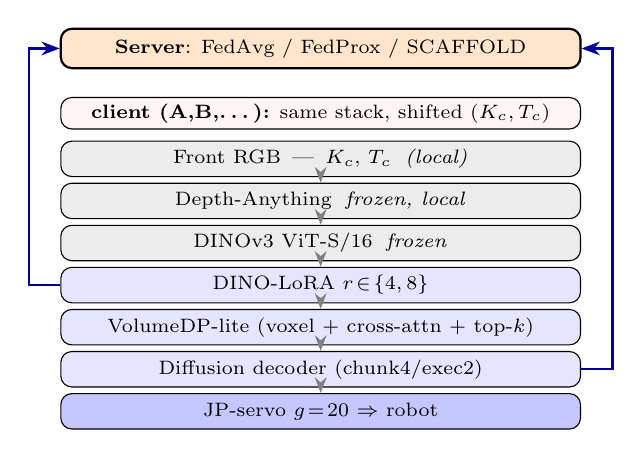
\begin{tikzpicture}[
  font=\scriptsize,
  box/.style={draw,rounded corners,minimum width=6.6cm,minimum height=0.45cm,
              align=center,inner sep=1pt},
  frozen/.style={box,fill=gray!15},
  trainable/.style={box,fill=blue!10},
  action/.style={box,fill=blue!22},
  server/.style={box,fill=orange!20,thick,minimum height=0.50cm},
  arr/.style={-{Stealth},semithick},
  uparr/.style={-{Stealth},thick,blue!60!black}
]
\node[server] (srv) {\textbf{Server}: FedAvg / FedProx / SCAFFOLD};
\node[box,fill=red!4,below=10pt of srv,minimum height=0.4cm] (lbl)
  {\textbf{client (A,B,\ldots):} same stack, shifted $(K_c, T_c)$};
\node[frozen,below=4pt of lbl] (cam) {Front RGB \,|\, $K_c$, $T_c$ \;\emph{(local)}};
\node[frozen,below=2pt of cam] (da)  {Depth-Anything \;\emph{frozen, local}};
\node[frozen,below=2pt of da]  (din) {DINOv3 ViT-S/16 \;\emph{frozen}};
\node[trainable,below=2pt of din] (lor) {DINO-LoRA $r\!\in\!\{4,8\}$};
\node[trainable,below=2pt of lor] (vol) {VolumeDP-lite (voxel + cross-attn + top-$k$)};
\node[trainable,below=2pt of vol] (dif) {Diffusion decoder (chunk4/exec2)};
\node[action,below=2pt of dif]    (act) {JP-servo $g\!=\!20$ $\Rightarrow$ robot};
\foreach \src/\dst in {cam/da, da/din, din/lor, lor/vol, vol/dif, dif/act}
  \draw[arr,gray] (\src) -- (\dst);
\draw[uparr] (lor.west) -- ++(-0.4,0) |- (srv.west);
\draw[uparr] (dif.east) -- ++(0.4,0)  |- (srv.east);
\end{tikzpicture}
\caption{Lightweight federated architecture. Frozen DINOv3,
Depth-Anything, the camera parameters $(K_c, T_c)$, and the
client-local voxel volume never leave the client. Only the LoRA
adapters, the VolumeDP cross-attention, and the diffusion decoder
($\sim$10\% of total parameters) are aggregated by the server.}
\label{fig:arch}
\end{figure}

\paragraph{Local-only (never communicated).}
Frozen DINOv3 and Depth-Anything weights (byte-identical, served
once at deployment); $K_c$, $T_c$, raw depth maps, and the
per-client voxel volume; optionally the diffusion action head
(personalised variant, see \S\ref{sec:agg}).

\paragraph{Server-aggregated ($\sim$10\% of params).}
DINOv3 LoRA matrices, the camera-ray and depth-fusion projector
MLPs, the VolumeDP-lite cross-attention and top-$k$ pooling
weights, and (in the standard variant) the diffusion decoder.

\subsection{Aggregation Scope: Four Variants}
\label{sec:agg}
A federated method is fully specified only when one decides
\emph{which} of the trainable modules are shared. With the two
ideas separated, the aggregation surface decomposes naturally:
\{LoRA + fusion projector\} comes from Idea~A, the volumetric
attention and top-$k$ pooling come from Idea~B, and the diffusion
decoder is shared by both. We compare four variants that
correspond to different combinations of \emph{what stays local}.

\noindent\textbf{V1 Global lightweight (baseline).} Aggregate
\{LoRA, fusion projector, volumetric attention, top-$k$ pooling,
diffusion decoder\}. The cheapest setting in which both ideas are
shared globally; fails when client demonstration styles are
heterogeneous because action heads are averaged.

\noindent\textbf{V2 Shared geometry / local action.} Aggregate
\{Idea-A LoRA, Idea-B volumetric attention\}; keep diffusion
\emph{decoder} client-local. Argument: after Idea~B's lift the
visual--geometric representation is shareable, but action heads
are sensitive to client-specific demonstration style, controller
gain, and timing. Closest to FedRep \cite{fedrep} applied to
manipulation.

\noindent\textbf{V3 Idea-A only (no Idea-B aggregation).}
Aggregate \{LoRA, fusion projector, decoder\}; keep the Idea-B
camera-aware projector and voxel attention \emph{client-local} so
they can absorb $(K_c, T_c)$ noise per client. This is the
right variant when extrinsics drift between sessions and we
cannot trust their alignment.

\noindent\textbf{V4 Staged personalisation.} Stage~1: aggregate
the Idea-A + Idea-B stack until convergence. Stage~2: freeze the
shared representation and fine-tune the diffusion decoder locally
for a small number of steps. Combines the best of V1 and V2.

\paragraph{Aggregator hypothesis.}
For each variant we compare FedAvg, FedProx, SCAFFOLD, with the
following hypothesis we want to falsify:

\begin{quote}\itshape
Idea~A removes backbone drift; Idea~B removes geometric
heterogeneity. Together they collapse the residual heterogeneity
to the point where FedAvg becomes competitive with SCAFFOLD on
the same surface, and FedProx's proximal term \emph{hurts}
because the LoRA-only aggregation surface is already small enough
that proximity regularisation over-restricts local adaptation.
\end{quote}

If both halves of the hypothesis hold, the contribution becomes
``an aggregation surface that no longer needs a heavy aggregator''
--- a stronger statement than ``a better aggregator''.

\section{Preliminary Experiments}
\label{sec:experiments}

All numbers are online success rate over 20 evaluation episodes.
Same-env probes use 50 epochs on \texttt{env0}; FL pilots use
10 rounds, fraction-fit~0.05. We run two complementary axes:
\textbf{task-level} (fix the FL setup, vary the visual / head
stack) and \textbf{federated-level} (fix the stack, vary the
camera shift / aggregator / aggregation scope).

\subsection{Task-Level Probes (Fixed FL Setup)}
\label{sec:task-probes}
Tab.~\ref{tab:slide-ablation} ablates the visual / head stack on
\emph{Slide Block} (env0). The decisive lift is the head
(MLP $\to$ diffusion); LoRA, depth, and gated proprio FiLM each
add a few points, taking the FLAME baseline 0.24 to 0.85.

\begin{table}[h]
\centering
\small
\caption{Task-level ablation, same-env on \emph{Slide Block}
(env0).}
\label{tab:slide-ablation}
\begin{tabular}{lc}
\toprule
Configuration & SR\\
\midrule
FLAME (CNN + MLP, FedAvg)         & 0.24\\
CNN + MLP (ours)                   & 0.40\\
DINO frozen + MLP                  & 0.40\\
DINO LoRA-4 + Diffusion            & 0.70\\
DINO LoRA-8 + Diffusion            & 0.70\\
DINO + Depth LoRA-8 + Diffusion    & 0.75\\
\,\,+ Proprio gated FiLM           & \textbf{0.85}\\
\bottomrule
\end{tabular}
\end{table}

\begin{table}[h]
\centering
\small
\caption{Same-env best per task vs.\ replay ceiling. \emph{Slide}
and \emph{Close} are policy-limited; \emph{Insert} and \emph{Scoop}
are limited by the absence of metric depth in the encoder, the gap
P3 (\S\ref{sec:plan}) is designed to close.}
\label{tab:sameenv}
\begin{tabular}{lccc}
\toprule
Task        & FLAME & Ours (best) & Ceiling\\
\midrule
Slide       & 0.24  & \textbf{0.85} & 1.00\\
Close Box   & 0.84  & 0.59          & 1.00\\
Insert      & 0.00  & 0.00          & 0.90\\
Scoop       & 0.00  & 0.20          & 0.90\\
\bottomrule
\end{tabular}
\end{table}

\subsection{Federated Pilot (Fixed Stack)}
\label{sec:fl-pilot}
A 10-round FedAvg/FedProx pilot on the LoRA-only surface
(without the volumetric module yet) confirms two things: the
diffusion head trains stably under FL (Tab.~\ref{tab:fl}), and
FedProx's proximal term hurts on this small aggregation
surface. The pilot is the launching point for the
camera-aware FL ablations (P3--P4).

\begin{table}[h]
\centering
\small
\caption{Federated pilot, 10 rounds, DINO LoRA-4 + Diffusion + JV
(no volumetric module yet).}
\label{tab:fl}
\begin{tabular}{lcc}
\toprule
Task        & FedAvg & FedProx\\
\midrule
Close Box   & \textbf{0.34} & 0.22\\
Slide Block & \textbf{0.16} & 0.04\\
\bottomrule
\end{tabular}
\end{table}

\subsection{Negative Result: Same-Env Camera-Aware Probe}
\label{sec:sameenv-camaware}

To verify that the FL contribution of Idea~B
(\S\ref{sec:idea-b}) does \emph{not} reduce to ``camera
parameters help any policy'', we trained the Idea-A+B stack on
\texttt{env0} with the same $(K_c, T_c)$ in every demonstration ---
a 33-DoF state ($8$ proprio + $9$ flattened $K_c$ + $16$
flattened $T_c$) replacing the 8-DoF baseline. Tab.~\ref{tab:camaware-sameenv}
shows that this lowers or fails to improve the SR on every task
where the baseline was non-zero.

\begin{table}[h]
\centering
\small
\caption{Same-env camera-aware probe vs.\ baseline (8-DoF state),
50 epochs on \texttt{env0}, 20 evaluation episodes. Adding
$(K_c, T_c)$ to the state \emph{hurts} when the camera is
constant across demonstrations, as expected.}
\label{tab:camaware-sameenv}
\begin{tabular}{lccc}
\toprule
Task & Baseline & Camera-aware (33-DoF) & $\Delta$\\
\midrule
Slide      & 0.85 & 0.20           & $-$0.65\\
Close Box  & 0.59 & 0.30           & $-$0.29\\
Insert     & 0.00 & 0.00           & $\pm$0\\
Scoop      & 0.20 & 0.00           & $-$0.20\\
\bottomrule
\end{tabular}
\end{table}

\noindent This is the predicted behaviour. Within a single
environment, $(K_c, T_c)$ is constant across every demonstration,
so feeding it to the policy adds no signal --- only dilutes the
head's capacity over a fixed dataset size. The corollary is
load-bearing for the proposal: \emph{Idea~B's contribution must
be evaluated under camera shift to be visible at all}. A same-env
probe is structurally insufficient to expose it; P3
(\S\ref{sec:plan}) is therefore the experiment that decides
Idea~B's federated claim, not the same-env tables.

\subsection{Same-Env Volumetric Probe: Idea~B's Actual Architecture}
\label{sec:sameenv-volumetric}

Tab.~\ref{tab:camaware-sameenv} added $(K_c, T_c)$ as flattened
state. To rule out the alternative explanation that the negative
result is an artefact of the trivial concat baseline, we re-ran the
same probe with Idea~B's actual proposed architecture: a frozen
DINOv3 + Depth-Anything dual stream lifted into a world-frame
voxel grid via $(K_c, T_c)$, with a TokenLearner-style softmax over
voxels into 48--96 spatial tokens, decoded by the same diffusion
head as the baseline. Volume bounds and grid resolution are the
two free parameters of the volumetric module; we sweep three
representative settings (Tab.~\ref{tab:volumedp-sameenv}). All
runs are 50 epochs on \texttt{env0}, 20 evaluation episodes, JV
direct.

\begin{table}[h]
\centering
\small
\caption{Same-env volumetric probe (Idea~B architecture, no $(K_c,
T_c)$ shift across demos). w1: default workspace volume
$[-0.45, 0.45]\!\times\![-0.55, 0.55]\!\times\![0.70, 1.35]$,
$12^3$ grid, 48 tokens. w2: same volume, $16^3$ grid, 96 tokens.
w3: tighter near-target volume
$[-0.30, 0.30]\!\times\![-0.40, 0.40]\!\times\![0.75, 1.10]$,
$12^3$ grid, 48 tokens.}
\label{tab:volumedp-sameenv}
\begin{tabular}{lcccc}
\toprule
Task        & Baseline & w1 (default) & w2 (grid16) & w3 (tight)\\
\midrule
Slide       & \textbf{0.85} & 0.20 & 0.65          & 0.05\\
Close Box   & \textbf{0.59} & 0.15 & 0.05          & --\\
Insert      & 0.00          & 0.00 & 0.00          & 0.00\\
Scoop       & \textbf{0.20} & 0.00 & 0.00          & 0.00\\
\bottomrule
\end{tabular}
\end{table}

\noindent Across all three volume settings the volumetric module
fails to recover the 2-D baseline on a single environment, with
the strongest variant (w2) reaching only $0.65$ on \emph{Slide}
versus $0.85$ from the proprio-FiLM baseline of
Tab.~\ref{tab:slide-ablation}. This is the predicted behaviour:
when $(K_c, T_c)$ is constant across demonstrations, the world-frame
lift produces the same voxel grid for every input and the
softmax-over-voxels module collapses to a learnt 2-D pooling whose
inductive bias does not match the data --- a strict regression
versus a CLS-token global pool. Together with
Tab.~\ref{tab:camaware-sameenv}, this rules out the trivialising
explanation that Idea~B helps only because $(K_c, T_c)$ adds free
state information; the volumetric machinery itself does
\emph{not} carry its own weight in the absence of camera shift,
which is exactly the load-bearing claim for the federated
experiments in P3 (\S\ref{sec:plan}).

\subsection{Evaluation Protocol Beyond Mean SR}
\label{sec:fl-metrics}
Mean SR alone does not capture federated performance. For all
P3--P5 experiments we report:
mean SR, \textbf{worst-client SR}, \textbf{client variance}
(std across clients), \textbf{communication cost} (MB / round /
client), \textbf{convergence round} (rounds to reach a target SR),
and the \textbf{same-env $\to$ multi-env gap} (a direct measure of
camera-induced robustness). The aggregation-scope study of
\S\ref{sec:agg} is meaningful only on these metrics, not on mean
SR alone.

\section{Discussion}
\label{sec:discussion}

\subsection{When Depth Helps the Task vs.\ When It Helps FL}
\label{sec:disc-task-vs-fl}
The same architectural component --- the depth-driven world-frame
voxel lift --- contributes to both axes, but for different reasons.
On the task axis, it gives the policy metric scale that monocular
RGB lacks; this is what makes \emph{Insert} and \emph{Scoop}
solvable in principle (replay ceiling 0.90, Tab.~\ref{tab:ceiling}).
On the federated axis, it converts client-frame observations into a
world-frame representation \emph{before} aggregation; this is what
makes the server's averaging well-posed. P2 and P3
(\S\ref{sec:plan}) test these two effects with separate ablations
so that we can attribute the gain correctly.

\subsection{Camera Intrinsics in Real Deployment}
\label{sec:fl-camera}
The single side-information our pipeline asks of each client is
$K_c$ and $T_c$. This assumption is essentially free in practice:
commodity RGB-D cameras (Realsense, Azure Kinect, ZED) ship with
factory intrinsics readable through the SDK; ROS standardises $K$
and distortion via \texttt{camera\_info}; intrinsics drift on
minute time-scales. Extrinsics $T_c$ are harder, drift faster, and
require workspace calibration; we consequently study a variant
(\S\ref{sec:agg} V3) that absorbs $T_c$ uncertainty in a local
adapter rather than treating $T_c$ as exact.

\subsection{Action-Servo Limitations}
\label{sec:disc-servo}
JP-servo still requires the demonstration to be reachable in JP
space. Tasks with explicit force-torque modulation cannot be
replayed by any kinematic interface; the 0.10 ceiling of EE-Plan on
\emph{Insert} hints at this regime. A force-aware action label is
left to future work; importantly, this is a task-level limit, not a
federated one, so it does not affect the FL conclusions of P3--P5.

\section{Plan and Deliverables}
\label{sec:plan}

\textbf{P1 Action-interface stabilisation (wk 1--2).} Migrate
\emph{Insert} / \emph{Scoop} to JP-servo $g\!=\!20$, sweep
$g\!\in\!\{10,20,30,40,60\}$. Target: $\geq\!0.5$ SR. Outcome
locks the action interface for all subsequent FL comparisons.

\textbf{P2 Idea-A vs Idea-B attribution (wk 3--4).} A
$2\!\times\!2$ ablation:
\{Idea~A on/off\} $\times$ \{Idea~B on/off\}. ``Idea~A off'' uses
a from-scratch CNN encoder; ``Idea~B off'' replaces voxel lifting
with a pooled image embedding. Same-env, fixed FL setup; measures
the \emph{task-level} contribution of each idea separately, so
that we can credit improvements to A, B, or their interaction.

\textbf{P3 Federated-level camera-shift study (wk 5--6).}
Re-run the $2\!\times\!2$ of P2 under three intrinsic-shift
schedules: \{none, $\pm10\%$ focal, $\pm10\%$ focal $+\,\pm\!5\,$cm
extrinsic\}. The hypothesis: as shift grows,
``Idea~A only'' (LoRA-only on a 2-D encoder) degrades; ``Idea~B
on top of Idea~A'' is approximately invariant; ``Idea~B alone, no
foundation backbone'' is between. Measures the \emph{FL-level}
contribution of camera-aware lifting beyond what Idea~A's frozen
backbone already provides.

\textbf{P4 Aggregation-scope ablation (wk 7--8).} The four
variants of \S\ref{sec:agg} (V1--V4) on the
front-only-with-shift setting. 30-round FedAvg / FedProx /
SCAFFOLD. Reports mean SR, \textbf{worst-client SR}, client
variance, communication cost. Tests the aggregator hypothesis of
\S\ref{sec:agg}.

\textbf{P5 Final tables and scaling (wk 9--10).} 4-task $\times$
all-method comparison; client-count scaling
$5/20/50/100/400$; communication budget plotted vs.\ SR. Stretch:
on-deployment $T_c$-noise robustness ablation.

{\footnotesize
\setlength{\bibsep}{0pt plus 0.3ex}
\bibliographystyle{icml2024}
\bibliography{proposal}
}

\end{document}
